%--------Pruebas del Sistema
%--------Daniel Ochoa John
%--------06/06/2012
\chapter{Pruebas del sistema}

En este capítulo se expondrán las pruebas realizadas al sistema utilizando experiencias reales de uso de una aplicación de pruebas por parte de usuarios voluntarios. Se describirá paso a paso el \textit{roadmap} que se ha adoptado para tales efectos.

\section{Pruebas de validación}

En esta sección se expondrán los resultados de una prueba de validación realizada en un ambiente controlado a la biblioteca desarrollada. Se ha utilizado la funcionalidad de exportar a XML los resultados obtenidos para evaluar, en primera instancia, si el comportamiento es acorde a lo esperado.

Para realizar esta prueba se han generado manualmente dos documentos XML de entrada, siguiendo el \textit{Schema} respectivo. Y se construyó una pequeña aplicación que haga las veces de aplicación cliente para la biblioteca, con la finalidad de poder realizar un \textit{merge} entre ambas fuentes.

La Figura \ref{fig:ps-im9} muestra el documento que se generó como representante para \textit{Facebook}, note que se trata de tres amigos (con datos reales del autor), que no son similares entre si. Estos amigos fueron seleccionados debido a que cumplen ciertas particularidades: uno de ellos es el que el autor considera como más cercano, otro es un contacto que en \textit{Twitter} tiene cuenta y sus nombres son muy similares y el tercero de ellos también cuenta con perfil en \textit{Twitter}, pero sus nombres no coinciden. Se puede apreciar mejor en la Figura \ref{fig:ps-im10}, que contiene el documento generado como representante para la Red Social de \textit{microblogging}.

\begin{figure}[H]
	\centering
	\includegraphics[scale=.7]{images/Figura6-9}
	\caption{\em Documento XML de prueba correspondiente a Facebook.}
	\label{fig:ps-im9}
\end{figure}

\begin{figure}[H]
	\centering
	\includegraphics[scale=.7]{images/Figura6-10}
	\caption{\em Documento XML de prueba correspondiente a Twitter.}
	\label{fig:ps-im10}
\end{figure}

En la aplicación cliente ha sido programado un \textit{merge} con \textit{k} igual a tres. Estos implica que, si el sistema está realizando los procesos correctamente, el documento XML de salida debería contener sólo tres contactos. 

Se espera que en el documento respectivo a \textit{Twitter} (Figura \ref{fig:ps-im10}), se descarte a "valirini" y a "shamirst" y que la información de "NRites" se una con la de "diegogutierrezmolina". Por otro lado, se espera que en el documento respectivo a \textit{Facebook}(Figura \ref{fig:ps-im9}), se seleccione a Valentina como el contacto más cercano y que la lista se complete con Diego y Shamir.

\begin{figure}[H]
	\centering
	\includegraphics[scale=.7]{images/Figura6-11}
	\caption{\em Documento XML resultado.}
	\label{fig:ps-im11}
\end{figure}


La Figura \ref{fig:ps-im11} muestra el documento que la aplicación de pruebas ha generado. Se puede apreciar que, efectivamente, Valentina es el contacto mas cercano al autor; Diego cuenta con información de ambas Redes Sociales y Shamir cierra la lista de tres sin su información de \textit{Twitter}. En conclusión, para esta experiencia la biblioteca parece funcionar correctamente, pero el escenario puede variar radicalmente cuando se ponga en práctica la segunda fase de pruebas. Este procedimiento se detalla en la sección siguiente.


\section{Concepción de pruebas al sistema}

Continuando con el plan de pruebas al sistema, llega el momento de evaluar su comportamiendo a gran escala, para esto se utilizó de un software que utiliza la biblioteca desarrollada en el capítulo anterior. Esta aplicación debe proporcionar información clara y estadística respecto a las relaciones existentes entre el usuario y sus contactos. Además, se contó con un grupo de usuarios voluntarios que han estado dispuestos a utilizar las aplicaciones de extracción con sus credenciales de inicio de sesión en las Redes Sociales, con el objetivo de tener acceso a la aplicación y obtener resultados. El proceso será realizado en una modalidad comparativa, para esto los usuarios contestaron una encuesta que contenía las siguientes preguntas:

\begin{enumerate}
\item ¿Cuáles son los contactos o amigos en las Redes Sociales con los que usted piensa que se relaciona más? Nombre 10 en orden decreciente. (Resultados esperados).
\item ¿Cree que se relaciona más con hombres o con mujeres?
\item Las relaciones pueden presentarse en distintos contextos, como laborales, familiares, educacionales o sentimentales (relaciones de pareja o amistades en general). De las 10 personas que seleccionó anteriormente, ¿en qué contexto usted considera que existe la mayor cantidad de relaciones? ¿En cuál menos?
\end{enumerate}

Posteriormente se utilizó la aplicación de pruebas para obtener la versión del sistema para las preguntas anteriormente descritas. Esta versión se comparó con la visión del usuario participante con el objetivo de obtener el porcentaje de éxito del sistema. Luego, los usuarios han elaborado un pequeño comentario respecto de la comparación entre los resultados esperados y los obtenidos, expresando su opinión respecto a por qué creen que se produjo diferencias, si las hubiese.


\section{La aplicación de pruebas}

El \textit{software} de pruebas que se utilizará se llama \textbf{RelationatorFX} y fue desarrollado en el contexto de este trabajo, bajo la plataforma \texttt{JavaFX}.
Esta aplicación recibe como parámetros de entrada los documentos XML obtenidos con las aplicaciones de extracción mencionadas en el capítulo cuatro. Luego, muestra información acerca de las relaciones del usuario en Redes Sociales suficiente como para abordar las preguntas anteriormente planteadas. La Figura \ref{fig:ps-im1} muestra la pantalla de inicio de RelationatorFX, en donde se puede apreciar los espacios de entrada para los documentos XML respectivos para \textit{Twitter} y \textit{Facebook} y el \textit{spinner} para asignar la cantidad de resultados que se desea obtener.

Las Figuras \ref{fig:ps-im2} y \ref{fig:ps-im3} muestran la pantalla principal del \textit{software} que expone, en modalidad de \textit{coverflow}, los k contactos más cercanos al usuario, junto con información de sus perfiles en las distintas Redes Sociales. Es importante notar que en la Figura \ref{fig:ps-im3} se puede apreciar la funcionalidad de detección de contactos similares ya que, para el contacto mostrado en la Figura \ref{fig:ps-im3}, se tiene información respecto a sus perfiles de \textit{Twitter} y \textit{Facebook}.

\begin{figure}[H]
	\centering
	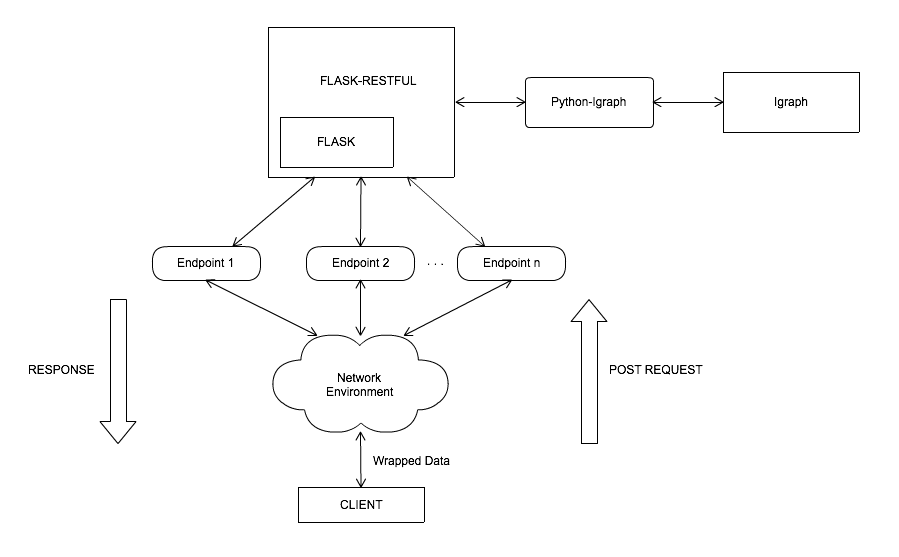
\includegraphics[scale=.4]{images/Figura6-1}
	\caption{\em Pantalla de inicio RelationatorFX.}
	\label{fig:ps-im1}
\end{figure}

\begin{figure}[H]
	\centering
	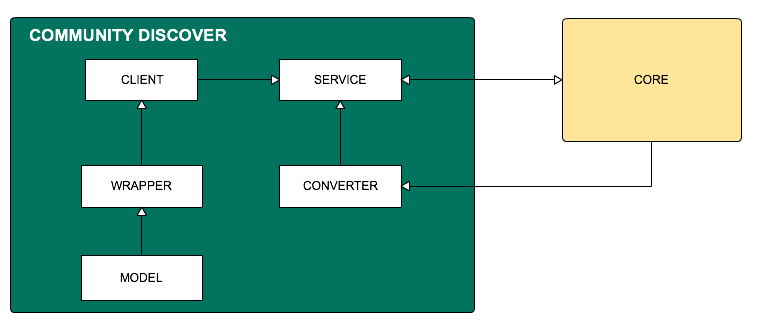
\includegraphics[scale=.4]{images/Figura6-2}
	\caption{\em Pantalla principal nº1.}
	\label{fig:ps-im2}
\end{figure}

\begin{figure}[H]
	\centering
	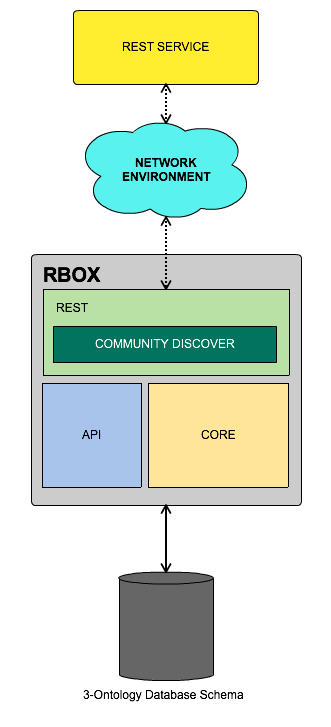
\includegraphics[scale=.4]{images/Figura6-3}
	\caption{\em Pantalla principal nº2.}
	\label{fig:ps-im3}
\end{figure}

Además, la aplicación grafica los resultados, generando información estadística. Entre los gráficos disponibles están:la curva de relaciones (\textit{Relatedness Chart}), que expone la parábola que forman los distintos grados de relación de los contactos; el gráfico de vista por géneros, que muestra en un gráfico de torta si se relaciona mayormente con hombres o mujeres; y finalmente, el gráfico de vista por contexto, que muestra el o los contexto/s a los que pertenecen los k-contactos más cercanos. Los gráficos se muestran en las Figuras \ref{fig:ps-im4},\ref{fig:ps-im5} y \ref{fig:ps-im6}.

\begin{figure}[H]
	\centering
	\includegraphics[scale=.4]{images/Figura6-4}
	\caption{\em Curva de relaciones.}
	\label{fig:ps-im4}
\end{figure}

\begin{figure}[H]
	\centering
	\includegraphics[scale=.4]{images/Figura6-5}
	\caption{\em Vista por géneros.}
	\label{fig:ps-im5}
\end{figure}

\begin{figure}[H]
	\centering
	\includegraphics[scale=.4]{images/Figura6-6}
	\caption{\em Vista por contextos.}
	\label{fig:ps-im6}
\end{figure}

El gráfico de la Figura 6-4 representa la curva de relaciones, en el caso de ejemplo señalado en la imagen se muestra una curva con una pendiente notoria entre el primer contacto y el segundo. Luego, la curva se regulariza asemejándose más a una recta. Esto implica que el primer contacto y el usuario se relacionan demasiado en Redes Sociales. La Figura 6-5 muestra que el usuario de ejemplo se relaciona más con mujeres que con hombres y, finalmente, el gráfico de la Figura 6-6 muestra que el contexto al cual pertenece la mayoría de los k-contactos obtenidos es el de educación.

Con esta información es posible proporcionar al usuario un parámetro suficiente para realizar una comparación respecto a los resultados que espera. Es en base a esto que se evalúa el porcentaje de éxito de la aplicación y la calidad de los resultados encontrados y, además, se obtienen situaciones interesantes respecto de las relaciones de las personas en las Redes Sociales. 


\section{Resultados obtenidos}

Se entrevistaron 10 usuarios y cada uno de ellos asumió un rol evaluador de la calidad de los resultados que el sistema entregó. Con las expectativas de respuesta, generadas al contestar la encuesta señalada en la Sección 6.2, como antecedentes, los usuarios generaron una ponderación de cada uno de los resultados obtenidos, de acuerdo a una escala de puntuación desde el número uno(el resultado más bajo), hasta el número cinco (el resultado más alto).  La Figura \ref{fig:ps-im7} siguiente muestra en un gráfico de torta la evaluación de los resultados obtenidos.

\begin{figure}[H]
	\centering
	\includegraphics[scale=.8]{images/Figura6-7}
	\caption{\em Evaluación de resultados.}
	\label{fig:ps-im7}
\end{figure}

El gráfico de la figura anterior muestra que la mayoría de los usuarios considera que las expectativas formadas respecto a sus contactos más cercanos coinciden precisamente con los resultados expuestos por el sistema. 
Un 35\% de los resultados arrojados por el sistema han sido catalogados como buenos, debido a que si bien los entrevistados consideraban dentro de sus posibles opciones a los contactos obtenidos, estos no aparecían en la posición correcta.
Se considera que la evaluación de la calidad de los resultados obtenidos es sobresaliente, ya que solo un 3\% de los contactos no formaban parte de la pre-concepción realizada por los usuarios evaluadores.
El 60\% de los usuarios entrevistados no era consciente de las relaciones que formó en sus Redes Sociales, ya que los resultados esperados coincidían muy poco con los resultados que el sistema obtuvo. Sin embargo, al ver los contactos que el sistema calculó como los más cercanos, inmediatamente el usuario se corregía y manifestaba que no había elegido bien los resultados que esperaba.
	En la Figura \ref{fig:ps-im8} se muestra un gráfico con la información expuesta por los usuarios respecto a la precisión con que la herramienta ha integrado los datos de contactos semejantes. Las opciones de correspondencia en unión de información se describen como: \textbf{coincide}, en caso de que se una de manera correcta la información correspondiente a \textit{Facebook} y \textit{Twitter}; \textbf{no aplica}, en caso de que un contacto seleccionado por el usuario solamente posea cuenta en una de las Redes Sociales, ya sea \textit{Facebook} o \textit{Twitter}; y \textbf{no coincide}, cuando al tener cuenta en ambas Redes Sociales, la información no se una correctamente.

\begin{figure}[H]
	\centering
	\includegraphics[scale=.8]{images/Figura6-8}
	\caption{\em Correspondencia en unión de información.}
	\label{fig:ps-im8}
\end{figure}

En el gráfico expuesto anteriormente se observa que para el 50\% de los contactos la información entregada por cada una de las Redes Sociales se une adecuadamente. Para un 48\% de los contactos los usuarios mencionaron que estos no poseían cuentas en ambas Redes Sociales, por lo que no aplica una unión de información. 
Es trascendental destacar el 2\% de no coincidencia de correlación de los datos, debido a que en estos casos los usuarios han mencionado que estos contactos no utilizan su nombre real en ambas Redes Sociales, recurriendo a sobrenombres en su lugar. Esto implica que al momento de realizar la evaluación de semejanza no sea posible obtener un grado de similitud entre ambas fuentes de información.
  
En el 20\% de los casos, los usuarios han mencionado que el sistema entregó resultados erróneos, es decir, mostraba contactos con los que el entrevistado no mantenía relación alguna. Estos contactos errados aparecen en los últimos lugares, en otras palabras,los contactos errados son los más lejanos.
Al momento de revisar, con el usuario siempre presente, el por qué de esta situación, la conclusión fue muy interesante: \textbf{el sistema no entregó resultados errados, sino que el usuario no tiene diez contactos cercanos}. 
Esto es, el entrevistado se relaciona en Redes Sociales con muy pocas personas de manera exclusiva, lo que provoca que las demás personas no tengan interacciones con el usuario más que los amigos en común, métrica que en esta anomalía fue determinante para seleccionar a estos contactos errados dentro del grupo de los \textit{k}-contactos más cercanos. 

